\documentclass{standalone}
\usepackage{tikz}
\usetikzlibrary{arrows.meta, positioning}

\definecolor{myblue}{RGB}{0, 0, 255} % Define blue color

\tikzset{
  mynode/.style={font=\small, inner sep=0pt},
  arrow/.style={-Stealth},
  bluepath/.style={draw=myblue, line width=1pt},
  blackline/.style={draw=black, line width=1pt, -stealth}
}

\begin{document}
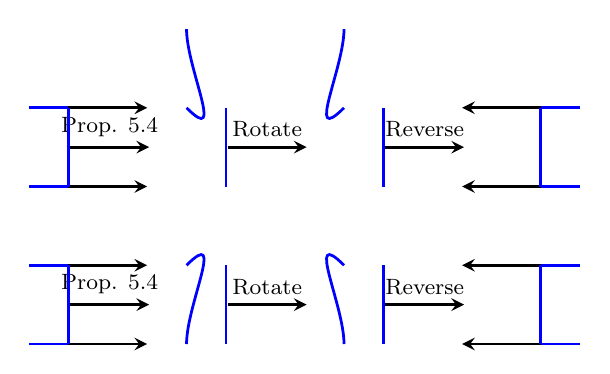
\begin{tikzpicture}[node distance=1.5cm]

% First Row
\node[mynode] (a1) at (0,0) {};
\draw[blackline] (a1.east) -- ++(1,0) node[midway,above] {\footnotesize Prop. 5.4};

\node[mynode] (b1) at (2,0) {};
\draw[bluepath] (1.5,0.5) .. controls +(0.5,-0.5) and +(0,-0.5) .. +(0,1);
\draw[blackline] (b1.east) -- ++(1,0) node[midway,above] {\footnotesize Rotate};

\node[mynode] (c1) at (4,0) {};
\draw[bluepath] (3.5,0.5) .. controls +(-0.5,-0.5) and +(0,-0.5) .. +(0,1);
\draw[blackline] (c1.east) -- ++(1,0) node[midway,above] {\footnotesize Reverse};

\node[mynode] (d1) at (6,0) {};

% Second Row
\node[mynode] (a2) at (0,-2) {};
\draw[blackline] (a2.east) -- ++(1,0) node[midway,above] {\footnotesize Prop. 5.4};

\node[mynode] (b2) at (2,-2) {};
\draw[bluepath] (1.5,-1.5) .. controls +(0.5,0.5) and +(0,0.5) .. +(0,-1);
\draw[blackline] (b2.east) -- ++(1,0) node[midway,above] {\footnotesize Rotate};

\node[mynode] (c2) at (4,-2) {};
\draw[bluepath] (3.5,-1.5) .. controls +(-0.5,0.5) and +(0,0.5) .. +(0,-1);
\draw[blackline] (c2.east) -- ++(1,0) node[midway,above] {\footnotesize Reverse};

\node[mynode] (d2) at (6,-2) {};

% Horizontal Lines for each row
\foreach \y in {0,-2} {
  \draw[bluepath] (-0.5,\y+0.5) -- (0,\y+0.5); % Left vertical line
  \draw[bluepath] (-0.5,\y-0.5) -- (0,\y-0.5);
  
  \draw[bluepath] (6,\y+0.5) -- (6.5,\y+0.5); % Right vertical line
  \draw[bluepath] (6,\y-0.5) -- (6.5,\y-0.5);
  
  \draw[blackline] (0,\y+0.5) -- (1,\y+0.5); % Horizontal lines
  \draw[blackline] (0,\y-0.5) -- (1,\y-0.5);
  
  \draw[blackline] (6,\y+0.5) -- (5,\y+0.5);
  \draw[blackline] (6,\y-0.5) -- (5,\y-0.5);
}

% Vertical Lines for each column
\foreach \x in {0,2,4,6} {
  \draw[bluepath] (\x,0.5) -- (\x,-0.5); % Top to bottom
  \draw[bluepath] (\x,-1.5) -- (\x,-2.5);
}

\end{tikzpicture}
\end{document}